\section{Linear Programming}

\subsection{Problem Formulation}

\begin{figure}[H]
\centering
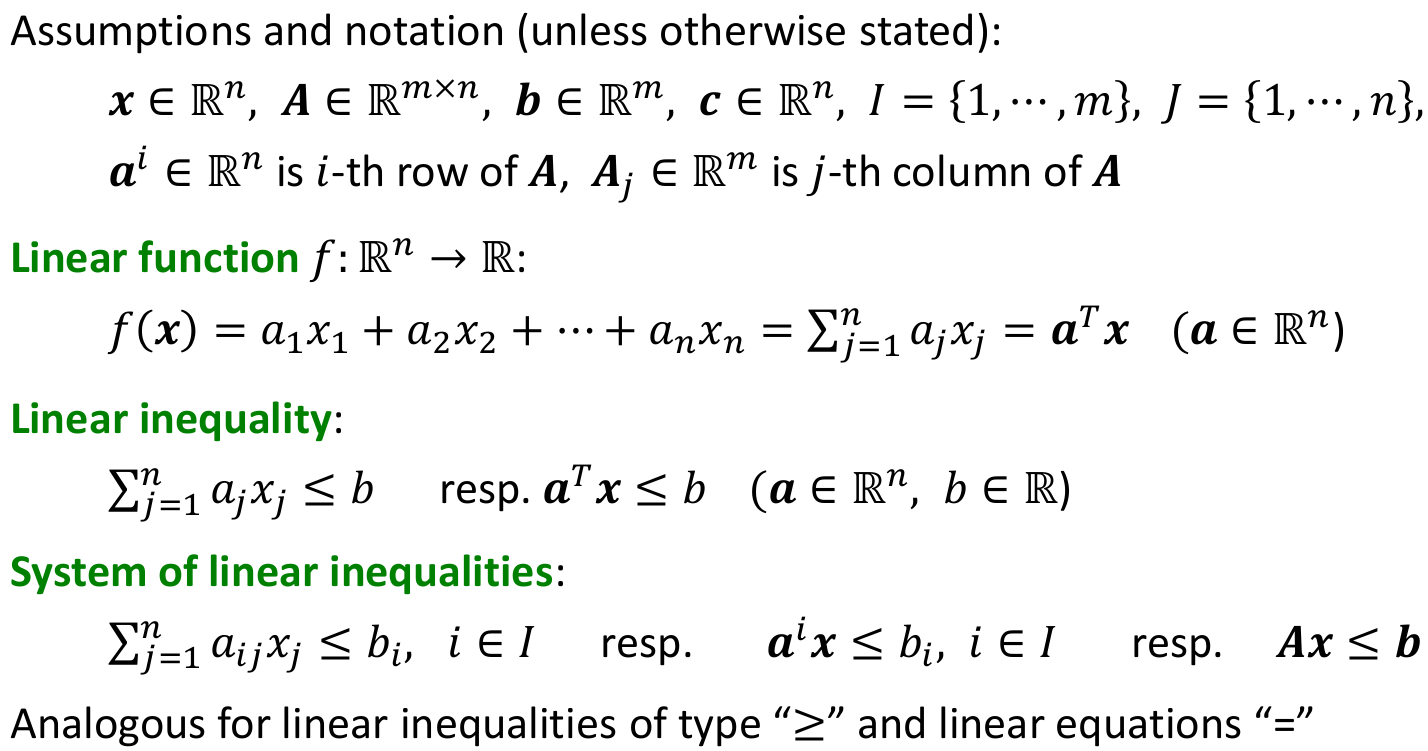
\includegraphics[width=0.5\textwidth]{figures/linearProgrammingProblemFormulation.png}
\caption{Linear Programming Problem Formulation}
\end{figure}

\subsubsection{Different Forms}
\begin{figure}[H]
\centering
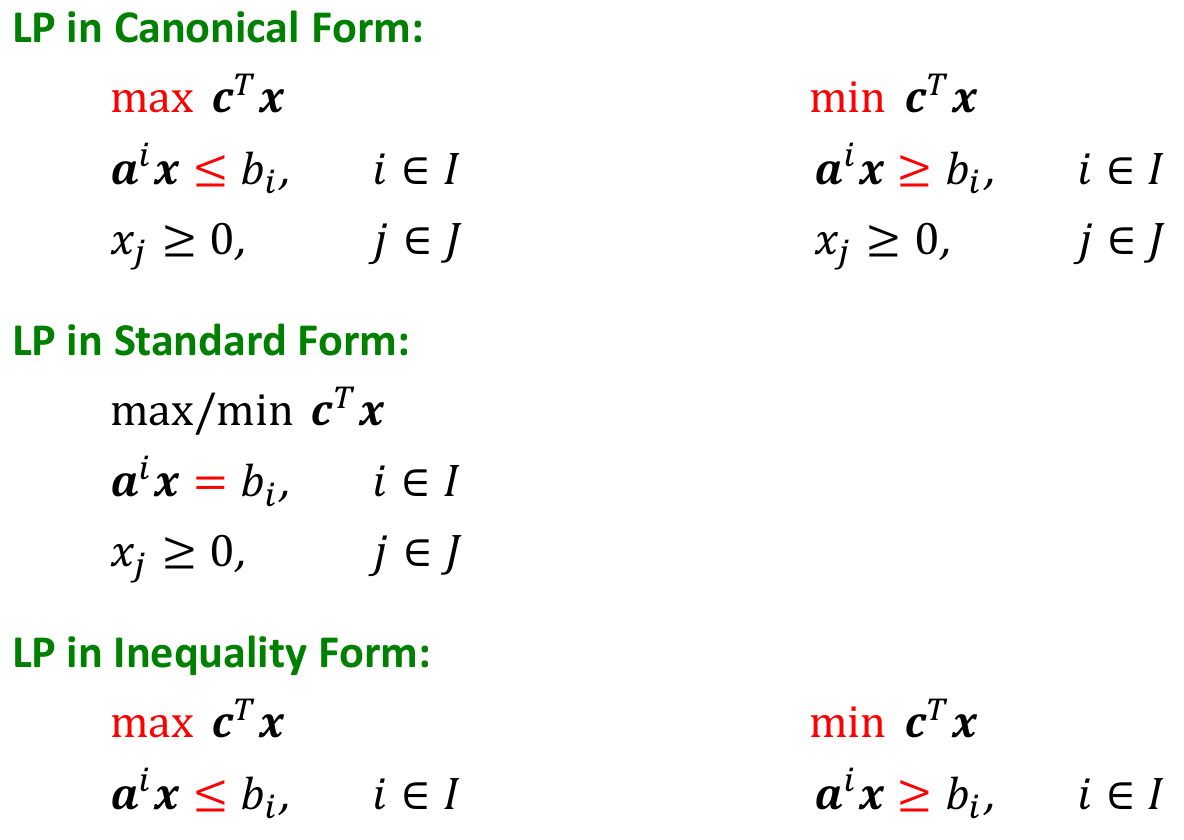
\includegraphics[width=0.5\textwidth]{figures/differentFormsLP.png}
\caption{Linear Programming - Different Forms}
\end{figure}

\textit{The inequality Form doesn't support any constraints.}

\subsubsection{Different Forms - Transformation}
\begin{figure}[H]
\centering
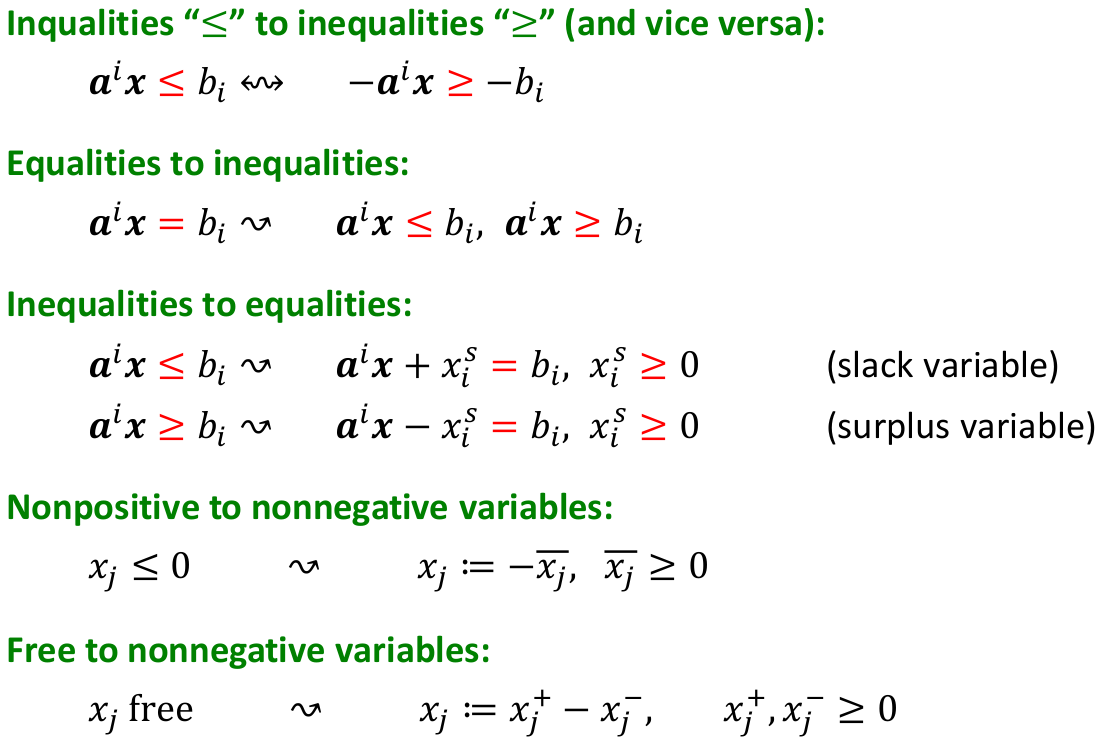
\includegraphics[width=0.5\textwidth]{figures/differentFormsTransformation.png}
\caption{Linear Programming - Different Forms - Transformation}
\end{figure}

\subsection{Geometric Aspects}

\begin{itemize}
    \item System of linear inequalities: $Ax \leq b$
    \item Linear inequalities $a^ix \leq b_i, i \in I$, are called linearly independend if vectors $a^i, i \in I$, are linearly independent.
    \item Analogous for $\geq$ and $=$.
    \item Let $A \in R^{m \times n}, b \in R^m$ and $B  \subseteq \{1, ..., m\}$. Define submatrix, subvector: $A_B = (a^i:i\in B)$ and $b_B = (b_i:i \in B)$
\end{itemize}

\textbf{Example:} \\
$A = 
\begin{vmatrix}
1&2 \\
5&3 \\
6&4 \\
\end{vmatrix}
=
\begin{vmatrix}
a^1 \\
a^2 \\
a^3 \\
\end{vmatrix}
,B = \{1,3\}$ then $A_B = 
\begin{vmatrix}
1&2 \\
6&4 \\
\end{vmatrix}
=
\begin{vmatrix}
a^1 \\
a^3 \\
\end{vmatrix}$

\subsubsection{Halfspaces and Hyperplanes}

\begin{figure}[H]
\centering
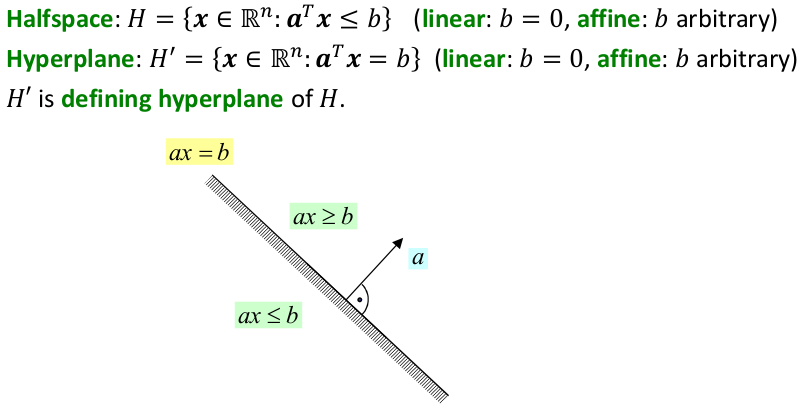
\includegraphics[width=0.5\textwidth]{figures/hyperplanes.png}
\caption{Definition of Hyperplanes}
\end{figure}

\begin{itemize}
    \item The Halfspace is the space which fulfills the inquality $a^Tx \leq b$
    \item The Hyperplane is the straight which splits the solution space between the halspace and the rest of the solution space
\end{itemize}

\begin{figure}[H]
\centering
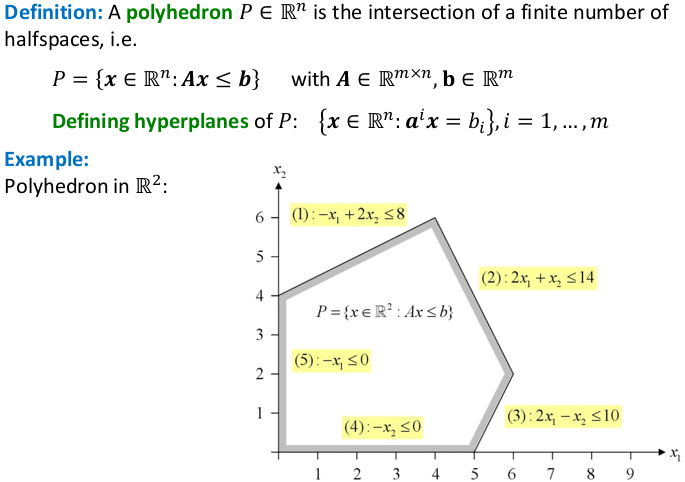
\includegraphics[width=0.5\textwidth]{figures/polyhedron.png}
\caption{Geometrics in a Polyhedron}
\end{figure}

\subsubsection{Basic Selection}
Let $P = \{x \in R^n:Ax \leq b\}$ with $A \in R^{m \times n}$ \\
A selection $B \subseteq \{1, ..., m\}$ of $|B| = n$ linearly independent rows of $A$ is called a \textbf{basic selection}, and the corresponding matrix $A_B$ is called a \textbf{basis} of $A$ \\
The vector $x = A_{B}^{-1} b_B$ is called the \textbf{basic solution} associated to basis $A_B$. \\
$B, A_B$ and $x = A_{B}^{-1} b_B$ are called \textbf{feasible} if $x \in P$.

\subsubsection{Geometric solution of LP's}

\begin{figure}[H]
\centering
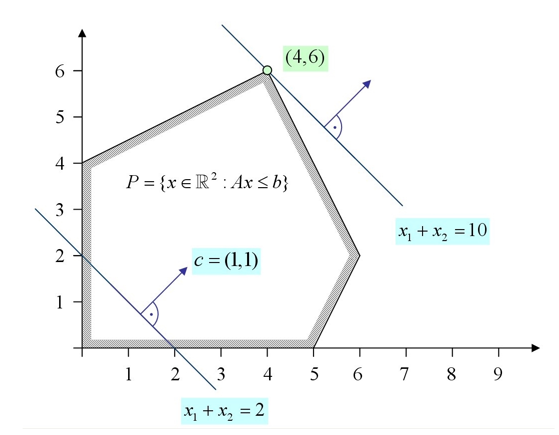
\includegraphics[width=0.5\textwidth]{figures/geometricLP.png}
\caption{Geometrics in a Polyhedron}
\end{figure}

We search the maximum at the corners of the polyhedron and walk along the edges till we find it. 

\subsection{Simplex Algorithm}

\begin{itemize}
    \item Das folgende Beispiel ist ein Körper im $R^2$, drei-dimensionalen Raum, mit drei Hyperplanes H.
    \item Jedes H hat einen Normalvektor a
    \item Um von der Ecke $v$ zu optimieren, müssen wir in die Richtung von $d$ also $v * \lambda d$ für $\lambda \geq 0$
\end{itemize}

\begin{figure}[H]
\centering
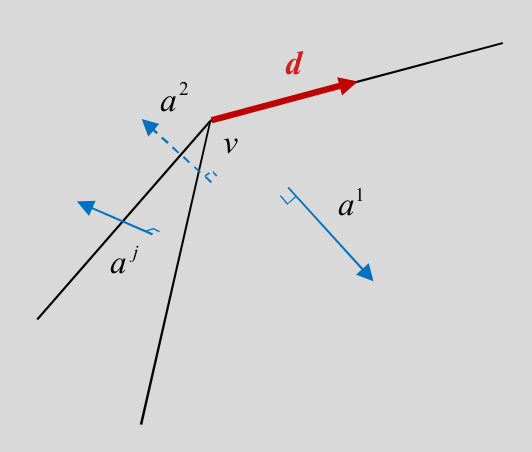
\includegraphics[width=0.4\textwidth]{figures/simplex_example.png}
\caption{Simplex Example}
\end{figure}

\begin{itemize}
    \item Wir müssen nun in die Richtung, die von den beiden Hyperplanes weg zeigt, von denen ich komme. 
    \item $d$ muss in die feasible direction zeigen $\Rightarrow \lambda a^j d \leq 0$ für $\lambda \geq 0$, daher $a^jd \leq 0$
    \item \textbf{$d$ ist also definiert als $d = -A_{j}^{-1}$}
    \item Wie lange können wir jetzt dieser Kante folgen?
    \item Der neue Punkt v' muss ebenfalls folgende Gleichung erfüllen: $A(v + \lambda d) \leq b$
    \item Daraus folgt, das grösstmögliche $\lambda = min\{\frac{b_i - a^iv}{a^id} : i \in I$ with $a^id > 0\}$
\end{itemize}

\subsubsection{Example}
$A(v*\lambda d) = Av + \lambda Ad = \begin{vmatrix}
7 \\ 11 \\ 2 \\ 4 \\ 8 \\ 9 \\
\end{vmatrix} + \lambda 
\begin{vmatrix}
3 \\ -2 \\ -1 \\ 0 \\ 2 \\ 5 \\
\end{vmatrix} \leq
\begin{vmatrix}
30 \\ 16 \\ 2 \\ 4 \\ 14 \\ 25 \\
\end{vmatrix}$

\textit{Alle Werte $\leq 0$ im Vektor bei $\lambda$ können wir ignorieren.}

\textbf{Minimum ratio test:} \\
$\lambda ' =  min\{\frac{b_i - a^iv}{a^id} : i \in I, a^id > 0\}$ = $min\{\frac{30-7}{3},\frac{14-8}{2},\frac{25-9}{5}$ = $min\{7\frac{2}{3}, 3, 3 \frac{1}{5}\} = 3$ (bei Index $i = 5$). \\
Der Index $i = 5$ ist jetzt die neue Ecke.

\textbf{\textit{Ich würde diesen Teil gerne nochmals repetieren.}}

\clearpage